\documentclass{standalone}
\usepackage{tikz}

\begin{document}

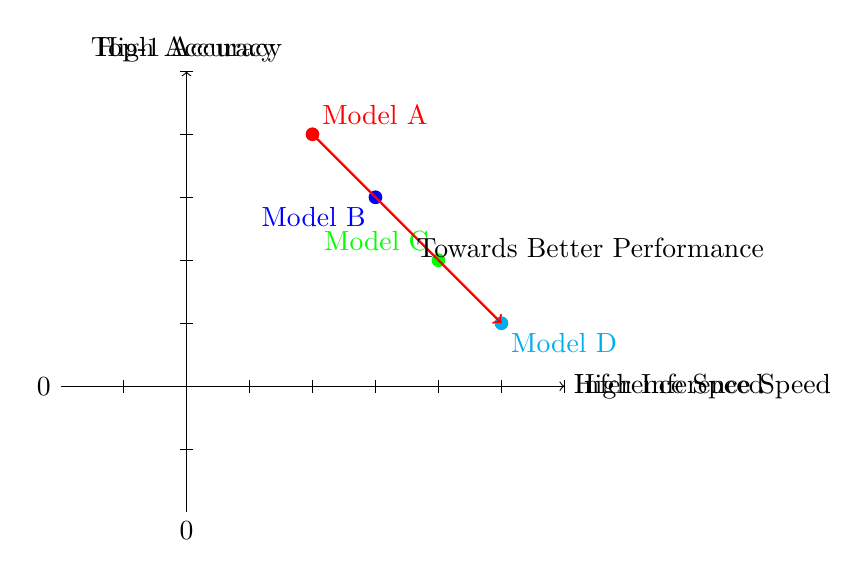
\begin{tikzpicture}[scale=0.8]
    % Axes
    \draw[->] (-2, 0) -- (6, 0) node[right] {Inference Speed};
    \draw[->] (0, -2) -- (0, 5) node[above] {Top-1 Accuracy};

    % Points with labels
    \filldraw[red] (2, 4) circle (0.1) node[anchor=south west] {Model A};
    \filldraw[blue] (3, 3) circle (0.1) node[anchor=north east] {Model B};
    \filldraw[green] (4, 2) circle (0.1) node[anchor=south east] {Model C};
    \filldraw[cyan] (5, 1) circle (0.1) node[anchor=north west] {Model D};
    
    % Arrows indicating improvement
    \draw[->, thick, red] (2, 4) -- (5, 1);
    \node at (3.5, 2.5) [below right] {Towards Better Performance};

    % Grid
    \foreach \x in {-1,0,...,6} \draw (\x,-0.1) -- (\x,0.1);
    \foreach \y in {-1,0,...,5} \draw (-0.1,\y) -- (0.1,\y);

    % Labels for axes
    \node at (-2, 0) [left] {0};
    \node at (0, -2) [below] {0};
    \node at (6, 0) [right] {High Inference Speed};
    \node at (0, 5) [above] {High Accuracy};

\end{tikzpicture}

\end{document}